\subsection*{Essencial}

\underline{NumPy} é um pacote para a linguagem Python que suporta arrays e matrizes multidimensionais, possuindo uma larga coleção de funções matemáticas para trabalhar com estas estruturas.

\begin{figure}[!htp]
    \centering
    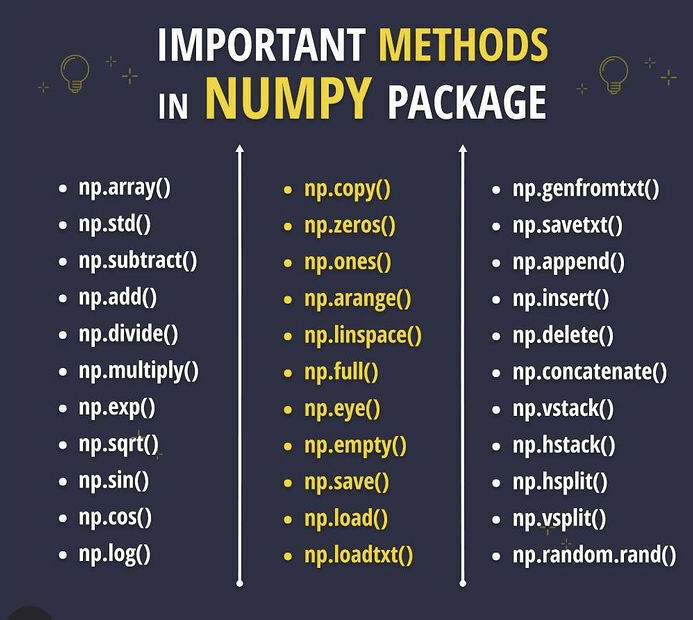
\includegraphics[scale=.8]{../img/python/numpy.jpeg}
    \caption{NumPy}
    \label{img:numpy}
\end{figure}


\underline{Pandas} é uma biblioteca de software criada para a linguagem Python para manipulação e análise de dados. 
Em particular, oferece estruturas e operações para manipular tabelas numéricas e séries temporais. 
O nome é derivado de painel data.

\begin{figure}[!htp]
    \centering
    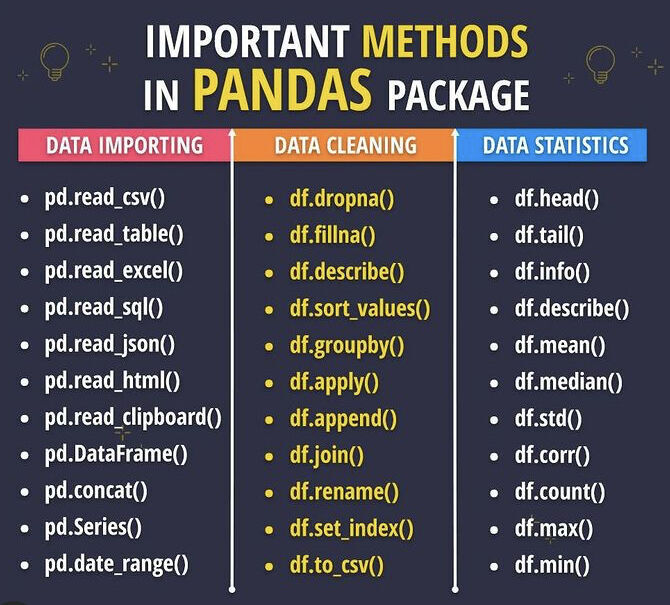
\includegraphics[scale=.8]{../img/python/pandas.jpeg}
    \caption{Pandas}
    \label{img:pandas}
\end{figure}
